\documentclass[a4paper,12pt,twoside]{report}
\usepackage{graphicx}
\usepackage{hyperref}
\usepackage[T1]{fontenc}
\usepackage[utf8]{inputenc}
\usepackage{setspace}
\usepackage[paper=a4paper,margin=1in]{geometry}
\usepackage[italian]{babel}
\usepackage{fancyhdr}

\title{Test Report}
\author{Davide Cologni}

\pagestyle{fancy}
\setlength{\headsep}{0.35in}
\let\MakeUppercase\relax
\renewcommand\sectionmark[1]{}
\setcounter{secnumdepth}{3}
\setcounter{tocdepth}{3}

\makeatletter
\let\inserttitle\@title
\let\insertauthor\@author
\makeatother

\begin{document}
    
    \begin{titlepage}
        
        \noindent
        \begin{minipage}[t]{0.19\textwidth}
            \vspace{-4mm}{
\includegraphics[scale=1.15]{logo_unimib.pdf}}
        \end{minipage}
        \begin{minipage}[t]{0.81\textwidth}
        {
                {\textsc{Università degli Studi di Milano - Bicocca}} \\
                \textbf{Scuola di Scienze} \\
                \textbf{Dipartimento di Informatica, Sistemistica e Comunicazione} \\
                \textbf{Corso di laurea in Informatica} \\
                \par
        }
        \end{minipage}
        
	\vspace{40mm}
        
	\begin{center}
            {\LARGE{
                    \textbf{\inserttitle}
                    \par
            }}
        \end{center}
        
        \vspace{50mm}

        \noindent
        {\large \textbf{Relatore:} Prof. Gainluca Della Vedova } \\

        \noindent
        {\large \textbf{Correlatore:} Dott. Antonio Riva}
        
        \vspace{15mm}

        \begin{flushright}
            {\large \textbf{Relazione della prova finale di:}} \\
            \large{\insertauthor} \\
            \large{Matricola 830177} 
        \end{flushright}
        
        \vspace{40mm}
        \begin{center}
            {\large{\bf Anno Accademico 2020-2021}}
        \end{center}
        
        \restoregeometry
        
    \end{titlepage}

    \tableofcontents
    
    \chapter{Introduzione}
    L'oggetto della tesi \'e una relazione dettagliata sul progetto di stage universitario svolto presso DDX,
    una software house che si occupa dello sviluppo di software CAD/CAM
    \footnote{\textbf{Software CAD/CAM} - Un software CAD/CAM è un programma che consente la progettazione (CAD)
    e la realizzazione (CAM) di manufatti in diversi materiali, come il legno, il vetro o la pietra, tramite 
    l'uso di macchine a controllo numerico (CNC).}.\\

    \begin{figure}[h]
        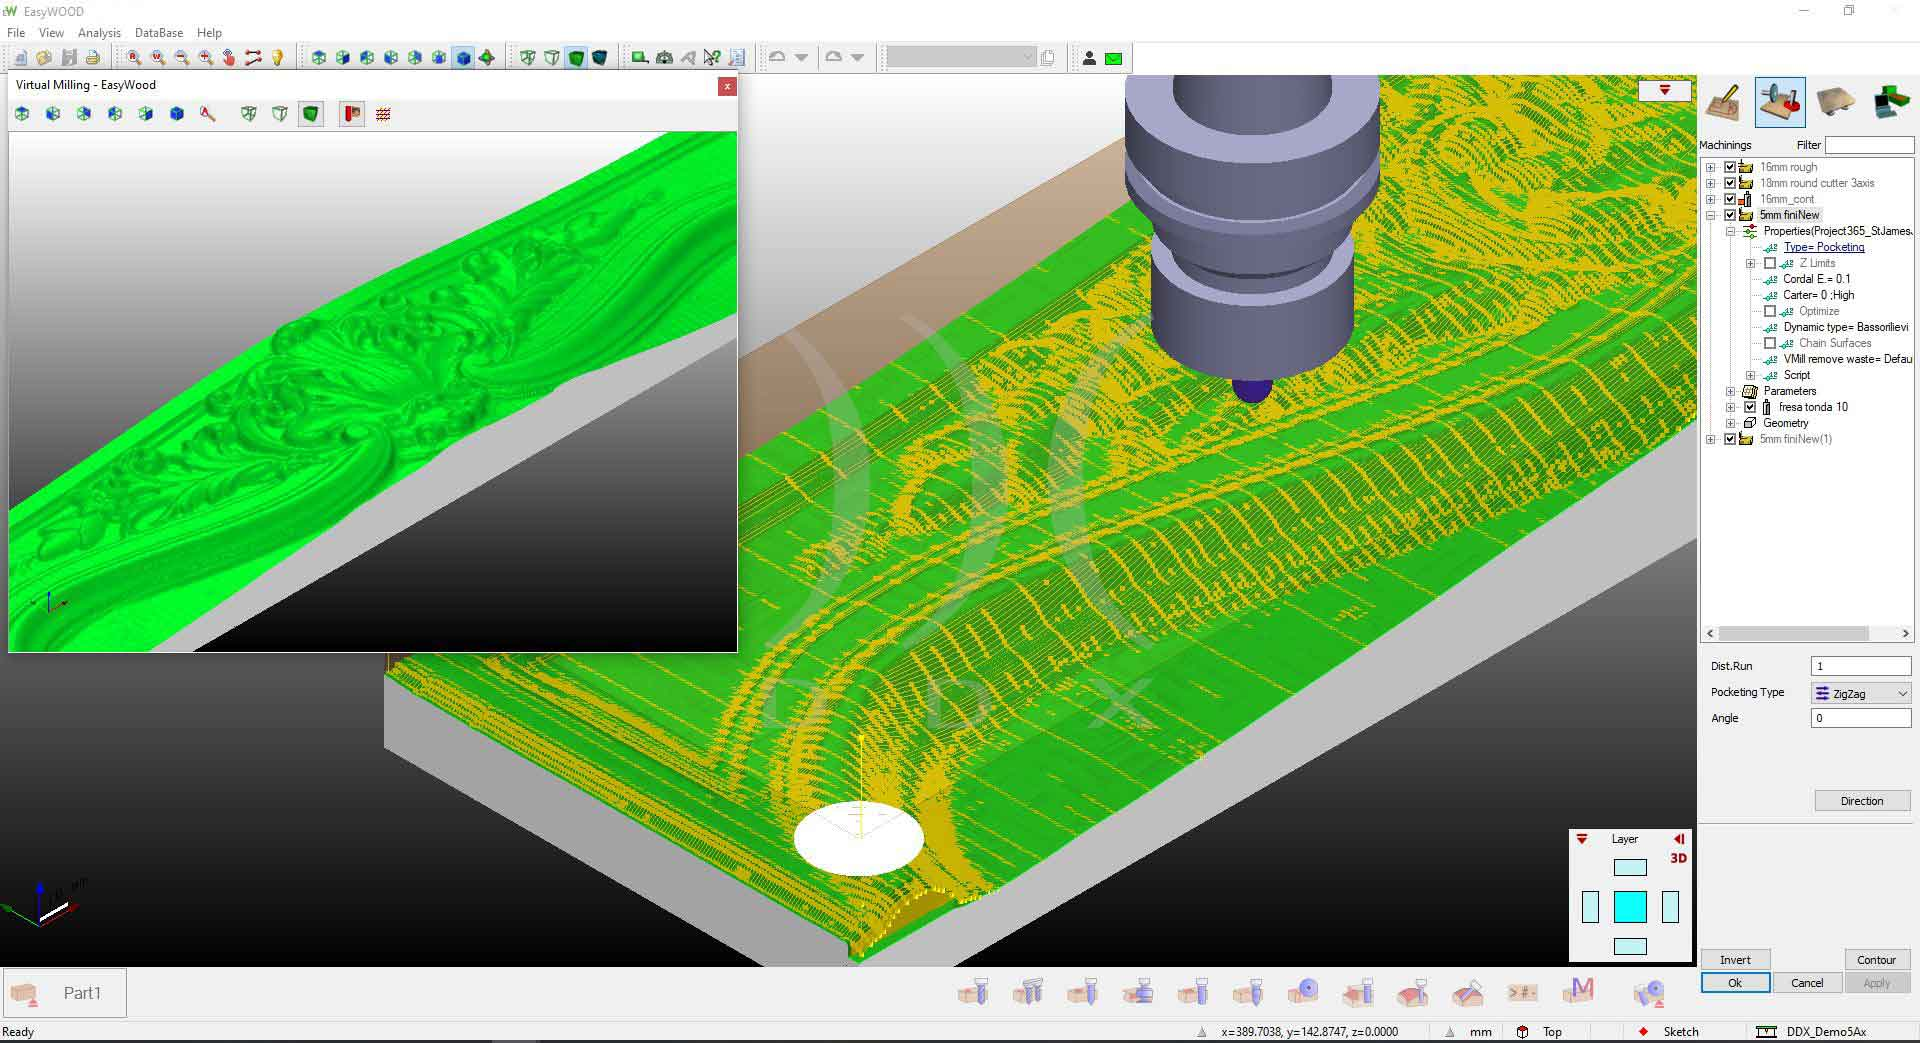
\includegraphics[width=\textwidth]{images/easywood.jpg}
        \caption{Uno dei Software di CAD/CAM sviluppato internamete}
    \end{figure}

    Il risultato questo periodo di sviluppo, durato in totale 3 mesi, \'e un report web dinamico per la consultazione e la modifica dei test. 
    In questa tesi verranno discusse le tecnologie, le scelte tecniche e la struttura dell'applicazione.\\

    Per essere meglio compreso il funzionamento dell'applicativo verr\'a illustrata nello specifico la struttura del sistema di test.\\
    Infine verr\'a descritta una panoramica del flusso di sviluppo e come il report in oggetto si integri con esso. 

    \chapter{Sistema di Testing}
    \section{Meccanismo dell'oracolo\label{oracolo}}
        Per la verifica del test viene sfruttato il meccanismo dell’oracolo.\\
        Esso consiste nell'accoppiare ogni test all'output corrispondente (chiamato appunto oracolo)
        e successivamente nell'effettuare un confronto tra il risultato del test e il suo riferimento.\\
        Il test viene dichiarato fallimentare se ci sono differenze tra gli outcome.\\
        
        Ogni test deve riferirsi solo a una funzionalit\'a o ad un insieme di esse strettamente correlate tra loro. \\
        Questo consente allo sviluppatore di individuare eventuali errori con maggiore precisione nel caso in cui un test fallisca. \\
        Se vi fosse la necessit\'a di cambiare le specifiche del software o di aggiungerne funzionalit\'a, \'e possibile rispettivamente modificare un oracolo esistente o crearne uno nuovo. \\

        Nel nostro sistema l'oracolo è salvato in un file \textit{.reference} e il risultato prodotto
        dal test in un file \textit{.current}.\\
        Il file current viene salvato nel file system solo nel caso in cui esso sia effettivamente diverso dal suo riferimento.\\
        
        Salvare il nuovo stato può consentire allo sviluppatore di confrontare i due file per capire quale sia l'errore introdotto nel software. \\
        Nella sezione successiva vengono illustrati gli elementi dal quale \'e composto un test e in seguito la loro funzione.\\
    \section{Anatomia di un test\label{testanatomy}}
        Un test consiste in un insieme di file locati per comodit\'a nella stessa cartella. \\

        Ogni test consiste in:
        \begin{itemize}
            \item Un file CAD di partenza
            \item Dei file per descrivere una configurazione specifica di un determinato cliente
            \item Un file SCL \footnote{\textbf{Sculptor Common Language} \'e un linguaggio di scripting proprietario interpretato con un insieme di routine per il disegno e la manifattura dei materiali} o un file python
            \item Uno o pi\'u riferimenti (file .reference)
        \end{itemize}

    \section{Ciclo di vita del test}
        Il software, per lanciare un test, importa il file CAD e le configurazioni del cliente.\\
        Successivamente esegue lo script SCL o Python, che con opportune librerie, si interfaccia con il software
        e simula le operazioni utente. \\
        
        Tra le diverse routine alcune si occupano di creare le reference esportando un risultato parziale dal programma come uno screenshot, un gruppo di entit\'a geometriche o un file testuale.

        Durante la esecuzione di un test i suoi outcome vengono salvati in una cartella di cache.\\
        Nel caso sia gi\'a presente una reference esso viene salvato come current.\\

        Se il file prodotto dalle operazioni \'e uguale all'oracolo, esso viene rimosso dal file system.\\
        In caso contrario il test \'e in stato di errore e l'output resta disponibile per il confronto.\\

    \section{Versioning dei tests}
            I test si trovano sotto un sistema di versioning.\\
            Quando uno sviluppatore decide di cambiare il comportamento di un caso d'uso o di aggiungere una funzionalità al software,
            sar\'a necessario modificare o creare un test.\\
            Esso verrà committato nel sistema di versioning in modo che gli altri sviluppatori possano testare il software secondo le nuove specifiche definite dal test.    


    \chapter{Struttura dell'applicazione}
    L'applicazione \'e stata sviluppata seguendo un'architettura client-server.
    
    Questa infrastruttura è composta da diversi programmi che interagiscono tra loro usando messaggi di rete, nel nostro caso codificati secondo il protocollo HTTP.
    Comunemente, le componenti principali sono il backend e il frontend.    

    \section{Elementi dell'applicazione}
        La prima componente di \textit{backend} si occupa della parte di logica di dominio dell'applicazione.
        La seconda, denominata \textit{frontend}, rappresenta graficamente i dati e di rende le interazioni tra essi gli stessi e l'utente fruibili.
        Decuplicare le parti dell'applicazione consente di rendere i singoli componenti riusabili.

        L'esempio pi\'u comune consiste nel condividere la logica dell'applicazione usando un backend e multiple rappresentazioni grafiche a seconda della piattaforma di utilizzo.
        In questo modo si può creare a un'applicazione web o un app mobile, senza duplicare la logica di dominio che verrà gestita dell'altra componente.
        
        Nel nostro caso in esame, la parte di backend si occuperà di leggere i test da file system e di esporli tramite un API.
        \'E stato sviluppato un frontend web per interagire graficamente con i test.

    \section{Intercomunicazione tra gli elementi}
        La comunicazione avviene tramite messaggi di rete codificati secondo il protocollo HTTP.
        La condivisione del protocollo consente agli attori di comunicare senza conoscere i dettagli implementativi dell'altro.
        Ci\'o implica un ulteriore vantaggio: gli elementi possono essere eseguiti su piattaforme diverse o essere scritti in linguaggi differenti, a seconda delle diverse necessità del singolo componente.
        
        Per il caso in oggetto la comunicazione viene iniziata dall'applicazione web e l'API REST si occupa di rispondere alle richieste.
        Il formato di interscambio dei dati usato \'e \textit{JSON}.

    \section{Vantaggi, svantaggi dell'architettura e alternative}
        I vantaggi di questa architettura, come precedentemente detto, sono la decuplicazione dei diversi elementi, il loro riutilizzo e la separazione delle responsabilità.
        
        In un caso futuro, sarà possibile sviluppare un altro frontend per visualizzare i test su un altra piattaforma riutilizzando il backend e garantendo la stessa logica applicativa.\\
        Viceversa la parte di frontend non conosce i dettagli implementativi usati dal backend come la gestione delle reference tramite file system e il sistema di versioning.\\
        Questo consente di cambiare le gestioni di basso livello lasciando invariato l'uso del programma agli occhi dell'utente.  
        
        Dall'altra parte, di contro, la separazione degli elementi porta a una piccola duplicazione di quelle che sono le parti comuni tra il client e il server, come i modelli di dominio.\\
        Per il tool aziendale precendente era stata adottata un'architettura diversa: un unico attore si occupava di consultare le reference e creare l'interfaccia grafica. \\
        Questo sistema non \'e per\'o estensibile e riusabile come quello attuale, essendo la logica di dominio e la generazione della pagina eseguita dallo stesso componente.


    \chapter{Backend}
        Il backend è stato sviluppato in \href{https://www.python.org}{Python} usando il framework \href{https://flask.palletsprojects.com/en/1.1.x/}{Flask}.
        \'E stato scelto Python perchè è un linguaggio già usato internamente per lo sviluppo di plugin e tool interni.

        \section{Specifica e documentazione}
            Prima della fase di sviluppo è stata predisposto un periodo di design dell' API.
            Questo processo ha prodotto un file di specifica (descritta nel paragrafo 
            \ref{openapi}).\\\\
            Questa fase preliminare allo sviluppo è durata circa una settimana ed è servita per 
            individuare difficoltà tecniche in modo preliminare che sono sate discusse con il team.
            Risparmiando così tempo in corso di sviluppo, evitando di dover ristrutturare l'applicazione.
            Questa specifica come vedremo in seguito è servita anche a produrre automaticamente una pagina di documentazione (\ref{apidoc}).
                
            \subsection{Specifica in linguaggio OpenAPI\label{openapi}}
                La Specifica dell'API è stata scritta in formato OpenAPI.
                Questo file può essere scritto in linguaggio JSON o YML, io ho scelto il secondo perchè
                sintatticamente più leggero e usa l'indentazione per separare le sezioni, facilitandone dunque la scrittura. 
                Questo formato ci consente di descrivere tutte le chiamate che il server 
                mette a disposizione, specificando:
                \begin{itemize}
                    \item il formato dell'URI 
                    \item il metodo
                    \item il formato di interscampio dei dati (json, xml ecc) 
                    \item la struttura del response 
                    \item come deve essere strutturato il body perchè la richiesta sia valida
                    \item i codici di errori e la loro semantica specifica nel contesto dell'applicazione
                \end{itemize}
                
            \subsection{Documentazione\label{apidoc}}
                Inoltre da questa specifica è possibile generare la documentazione, in pagina statica html,
                tramite l'utilizzo di diverse cli.
                Io ho scelto ReDoc, perchè mette a disposizione diverse vendore-extension, cioè sezioni che
                se specificate provedono una maggiore customizzazione della pagina generata, come sezioni di codici disposizione
                esempio per effettuare una determinata chiamata al server.
                Oppure aggiungere riferimenti a file markdown esterni da includere nella documentazione.
                
            \subsection{Continous integration}
                Il processo di scrittura della documentazione è stato aggiunto a una pipeline di CI
                \footnote{\textbf{Continous Integration} - L'integrazione continua consiste nell'integrare gli ambienti di sviluppo dei diversi sviluppatori tramite processi di build, testing ecc... eseguiti da un server condiviso}.
                Questo processo si occupa, solo se il file .yml di specifica viene modificato, di 
                rigenerare il file html di documentazione.
                Questo file viene successivamente servito in modo da rendere la documentazione 
                disponibile online e sempre aggiornata con le specifiche.

    \section{Tecnologie Utilizzate}  
        \subsection{Python}
            Python \'e un linguaggio di scripting, interpretato ad alto livello, ovvero la gestione della memoria viene effettuata da un sistema di garbage collection e non delegata allo sviluppatore.
            L'uso di python è dovuto al fatto che \'e un linguaggio gi\'a usato per lo scripting all'interno dell'applicazione e dunque gi\'a familiare a motli sviluppatori.
            Tra le varie librerie prodotte \'e presente anche un modulo per lanciare i test e inviare i risultati agli sviluppatori via e-mail.
            Questo modulo non è stato utilizzato all'interno del test report l'uso dello stesso linguaggio ha contribuito a mantenere la code-base pi\'u uniforme.
        \subsection{Flask}  
            Flask \'e un \textit{micro}Framework per la creazione di servizi web, esso consente di creare applicazioni complete o API (come nel nostro caso)
            La sua peculiarit\'a \'e la sua minimalit\'a e consente si scrivere applicazioni in modo rapido riducendo al minimo la parte di codice che si occupa della gestione dell'interfaccia HTTP, usando gli strumenti di introsprezione del codice offerti dal linguaggio come i decoratori.
            Esso \'e stato scelto perch\'e l'applicazione non necessitava di gestioni di basso livello riguardo la comunicazione di rete, ma la parte pi\'u importante dell'applicazione era l'attraversamento del file system per collezionare le informazioni riguardo ai test e l'interfaccia con i sistemi di versioning.

    \section{Implementazione interna}
        \subsection{Interazione con i sistemi di controllo di versione}
                
            TODO: dire che quando i test sono committati la stage e l'implementazione della stage per svn.

            Tutte le azioni effettuate dal report sono operazioni sul file system dunque sono completamente reversibili, e esse non sono definitive fino a quando non viene espressamente effettuato un commit.\\
            Una specifica del report \'e poter usare sia \textbf{Git} e \textbf{Svn (Subversion)} in modo trasparente allo sviluppatore.
            Questo perch\'e in futuro si prevede di migrare la suite di test sa Subversion a Git.
    
    \section{Bundling dell'applicazione e deploy}
        TODO: Spiegare come l'ho messo sul server

        In produzione l'applicazione serve l'API e il frontend sulla stessa porta.
        Questo è stato fatto separando il metodo di risoluzione delle root in due, per prima gli indirizzi che iniziano con \textit{v1/} contengono gli end-point del frontend
        Gli altri indirizzi si occupano di servire il frontend, essi son stati a loro volta suddivisi:
        I file statici (detti assets) e le route della Single Page Application.
        Se il percorso coincide con uno presente nella cartella \textit{static} viene servito il file trammite HTTP
        Altrimenti viene servito il file HTML index che essendo una single page application si occuper\'a di reindirizzare l'utente sulla pagina richiesta o di segnalare errore
    
    \chapter{Frontend}
    \section{Angular}
        \subsection{Scelta dell'utilizzo}
            \'E stato scelto di usare Angular, perchè è un framework stabile supportato da Google
            e \'e già stato usato precedentemente per lo sviluppo di altri applicativi.
            
            La struttura a componenti, favorisce il riuso del codice perciò è stato possibile integrare
            nello sviluppo componenti già sviluppati da altri, che forniscono comportamenti base
            come il rendering 3d di un file CAD proprietario.
        
        \subsection{Typescript}
            Un altro motivo per la scelta di Angular è \href{https://www.typescriptlang.org}{Typescript}.
            Typescript è un \textit{superset di javascript} cioè una sua estensione che ingloba tutte le sue feature e ne aggiunge altre.
            La sua peculiarità principale è l'aggiunta di uno step di compilazione che consente di aggiungere una tipizzazione statica.
            Questa tipizzazione consente allo sviluppatore di
            \href{https://www.quora.com/Why-is-type-checking-important-in-programming-languages-and-how-should-one-choose-between-dynamically-and-statically-typed-languages}{ridurre errori banali}.
    \section{Funzionalità}
        \subsection{visualizzazione dei test}         
        \subsection{Gestione interattiva dei file stageati}         
        \subsection{Modalità compatta}
        \subsection{Navigazione}
            E\'  disponibile un metodo di navigazione per aumentare l'usabilità dell'applicazione.
            Durante la navigazione è possibile rendere un test \textit{focussed} e effettuare operazioni (come nasconderlo o metterlo in stage) usando delle scorciatoie da tastiera.\\
            Si può spostare il focus sul test precedente e successivo sempre usando shortcuts.
            Solo un test può essere in focus.\\
            Quando il focus si sposta su un nuovo test la pagina effettua un operazione di scroll per renderlo visibile e scrive il suo nome nell'url, nella sezione denominata \textit{fragment}.\\
            Se la pagina viene richiesta con un fragment già impostato, in fase di rendering dei tests viene focussato automaticamente il test con quel nome (e quindi incluso nella sezione visibile della pagina).\\
            Questo consente agli utenti di condividere un test trammite url.

            TODO: immagine test navigazione e url con fragment
    \section{Interazione con gli altri tool aziendali}
    
    \chapter{Uso nel processo di sviluppo}
    
    \chapter{Sviluppi Futuri}
    \section{Migrazione test suite da svn a git}
    \section{Performance dei test}
    \section{Differ integrato}

    \chapter{Conclusioni}
    \section{Risultato finale e obiettivi iniziali}
    In questa tesi \'e stato descritto il software "Test Report" per l'analisi e accettazione dei test.\\
    Nel corso di questo trattato \'e stata posta l'attenzione sui concetti quali l'architettura REST, l'importanza del processo di testing e l'uso degli strumenti di sviluppo come l'integrazione continua e i sistemi di revisione del software.\\

    Il progetto \'e riuscito a soddisfare tutti i punti necessari definiti dalle specifiche iniziali.\\
    Inoltre nel periodo di stage \'e stato possibile anche distribuire il progetto in produzione su tutti i server di test.\\

    \section{Ringraziamenti}
    
    Un ringraziamento speciale al mio relatore Gianluca Della Vedova, per la sua pazienza e disponibilit\'a.\\

    Ringrazio il mio correlatore Antonio Riva per l'aiuto datomi e l'entusiasmo trasmesso durante il periodo di stage.\\

    Un ulteriore ringraziamento va alla mia famiglia che mi ha sempre supportato, in particolar modo a mia nonna Angiolina e a mia nonna Anna che sono state un esempio di cura e di amore.\\
    A loro voglio dedicare questa tesi.\\

\end{document}
            